% 
% Annual CCN conference
% Sample LaTeX Two-Page Summary -- Proceedings Format
% based on the prior cognitive science style file

% Original : Ashwin Ram (ashwin@cc.gatech.edu)       04/01/1994
% Modified : Johanna Moore (jmoore@cs.pitt.edu)      03/17/1995
% Modified : David Noelle (noelle@ucsd.edu)          03/15/1996
% Modified : Pat Langley (langley@cs.stanford.edu)   01/26/1997
% Latex2e corrections by Ramin Charles Nakisa        01/28/1997 
% Modified : Tina Eliassi-Rad (eliassi@cs.wisc.edu)  01/31/1998
% Modified : Trisha Yannuzzi (trisha@ircs.upenn.edu) 12/28/1999 (in process)
% Modified : Mary Ellen Foster (M.E.Foster@ed.ac.uk) 12/11/2000
% Modified : Ken Forbus                              01/23/2004
% Modified : Eli M. Silk (esilk@pitt.edu)            05/24/2005
% Modified : Niels Taatgen (taatgen@cmu.edu)        10/24/2006
% Modified : David Noelle (dnoelle@ucmerced.edu)     11/19/2014
% Modified : Konrad Kording (koerding@gmail.com)     2/15/2017
% Modified : Thomas Naselaris (tnaselar@gmail.com)   3/18/2022
% Modified : Sneha Aenugu & Jasper van den Bosch   18/12/2024

\documentclass[10pt,letterpaper]{article}

\usepackage{ccn}
\usepackage{pslatex}
\usepackage{apacite}
\usepackage{graphicx}
\usepackage{hyperref}
\hypersetup{colorlinks=false,breaklinks=true}


\title{Surveying Current Performance on Long Range Visual Reasoning}

\author{{\large \bf Anonymous authors} \\
Double blind review}
 
% \author{{\large \bf A Person (Person@this.planet.edu)} \\
%   A Department, 1234 Example Street\\
% A City, State 12345 A country
%   \AND {\large \bf Another Person (AnotherPerson@this.planet.edu)} \\
%   A Department, 1234 Example Street\\
% A City, State 12345 A country}


\begin{document}

\maketitle


\section{Abstract}
{
\bf
The appearance of new mechanisms for neural networks, including the attention architecture and state space models, has led to an explosion of new vision models able to compete with or beat previous state of the art approaches on a variety of tasks. The performance of these new models on long-range visual reasoning tasks – and the ability of these models to generalize to longer reasoning broadly from specific domains of computer vision – remains an open question. We created a model zoo, including CNNs, ViTs, ConvViTs, and RNNs, to measure performance on a range of long-range visual reasoning tasks, demonstrating that despite improvements from the long context-windows of transformers over traditional CNNs, these models still struggle on long-range tasks. These results indicate that the representational requirements for tasks like image recognition might be distinct from long-range visual reasoning and the latter are still imperfectly represented in current machine learning models, despite strong performance on traditional computer vision tasks.
}
\begin{quote}
\small
\textbf{Keywords:} 
long-range spatial reasoning; transformers; convolutional neural networks; long-range arena
\end{quote}

\section{Introduction}
Long-range visual reasoning, or the ability to solve tasks that require integrating information across spatial distance, is a fundamental component of visual intelligence. These capabilities are present in such trivial cognitive activities as tracing a path on a subway map or identifying complex patterns. Theories of visual perception have proposed a distinction between parallel, feedforward grouping of local features and serial, attention-demanding grouping of spatially distant elements (Houtkamp \& Roelfsema, 2010). This raises the question of whether current vision models, trained primarily on tasks amenable to local feature detection, have learned representations sufficient for the latter.

In machine learning, the goal of modeling long-range dependencies has driven the creation of both novel model architectures and benchmarks to measure the performance of models on long-range reasoning. The latter include the Pathfinder and "cluttered ABC" (cABC) tasks, which originated in cognitive psychology; Pathfinder has since been incorporated into the Long-Range Arena as part of an attempted systematic and unified benchmark for transformers' performance (Linsley et al., 2018; Kim et al., 2020; Tay et al., 2021).

Such new benchmarks are necessary in part due to the rapid appearance of new models, built off of new architectural approaches beyond traditional convolutional neural networks. The Long-Range Arena focused on transformer architectures, which now include Vision Transformers (ViTs), but state-space models (SSMs), a development on recurrent neural networks, have also become competitors for transformers in this space (Dosovitskiy et al., 2021; Gu et al., 2022).

\begin{figure}[ht]
% \begin{center}
% \fbox{CCN figure}
% \end{center}
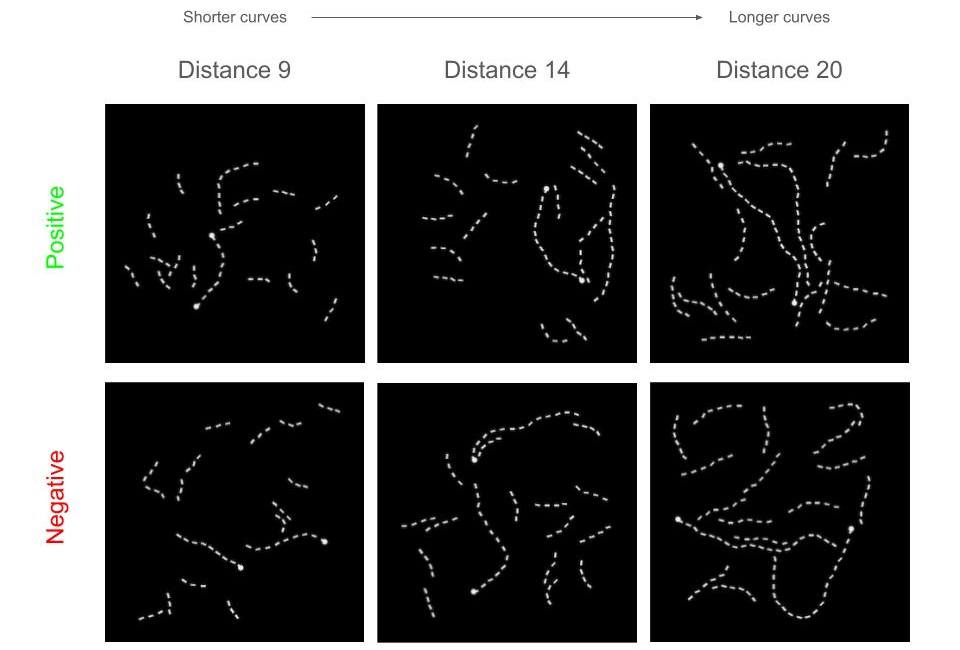
\includegraphics[width=\linewidth]{PF ex.jpg}
\caption{In the Pathfinder task, participants must determine whether two white markers fall on the same or different path. The difficulty of this task is parametrically controlled by the length of the target curve.} 
\label{Pathfinder-Graphic}
\end{figure}

\begin{figure}[ht]
% \begin{center}
% \fbox{CCN figure}
% \end{center}
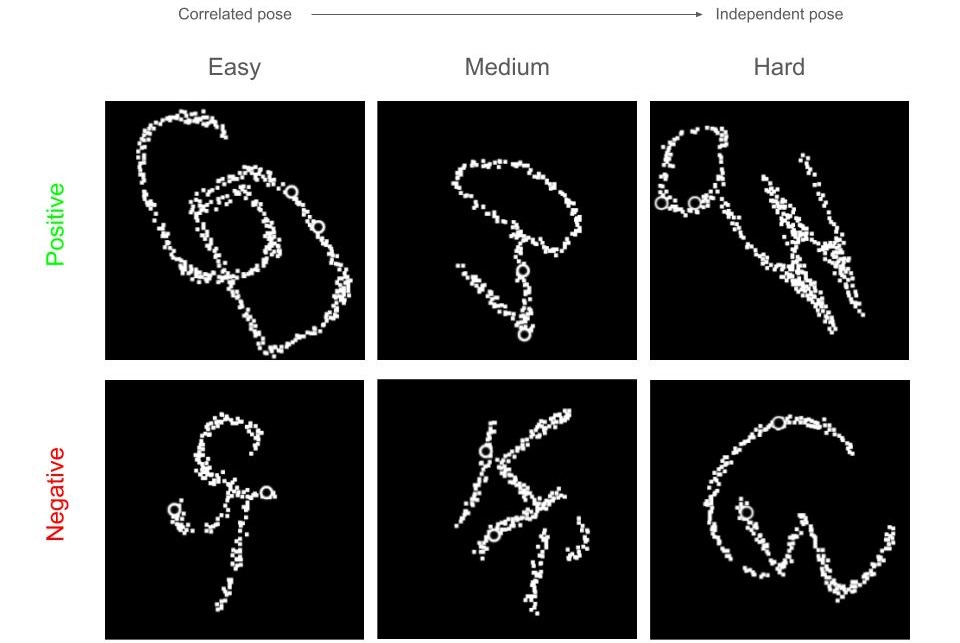
\includegraphics[width=\linewidth]{cABC ex.jpg}
\caption{In the cABC task, participants must determine whether two white markers fall on the same or different letter. The difficulty of this task is parametrically controlled by decreasing the correlation between geometric transformations applied to the two letters while increasing the
relative positional variability between letters.} 
\label{cABC-Graphic}
\end{figure}

\section{Methods}

We used the PyTorch Image Models (timm) collection as a source for a variety of pre-trained image models with known performance on a major computer vision task, in this case ImageNet (Wightman et al., 2021). For each model, we trained a linear probe on the model's representations from each task to determine whether the model had learned long-range dependencies in the course of model pre-training.

For the evaluation tasks, we used Pathfinder and cABC. Both tasks come with demarcated difficulties, based on the distance required for a reasoner to traverse to solve the task. We trained and evaluated linear probes at each difficulty level independently, allowing us to observe how performance degrades as the spatial range required for the task increases.
% For this paper, we varied both the training and testing difficulties, training linear probes on a particular difficulty and testing on that same difficulty, rather than training exclusively on the hardest difficulty and testing on lower difficulties; unlike fixed-difficulty benchmarks where local shortcuts may suffice, we varied task difficulty to stress long-range integration.

Linear probing provided two benefits for our research. First, as a matter of scale, it allowed us to maximize the number of models that could be included in the model zoo. Second, training from scratch has been shown to grossly overestimate differences between architectures (Amos et al., 2024); our use of pretrained representations avoids this confound while also testing whether general vision competencies generalize to long-range reasoning.
% Second, while initializing randomly and training from scratch, which has been demonstrated to bias the priors in favor of specific architectures (Gupta paper?), training linear probes allowed us to directly measure if general vision competencies -- in this case, image recognition -- generalizes to logical reasoning.

\section{Results}

\begin{figure*}[ht]
% \begin{center}
% \fbox{CCN figure}
% \end{center}
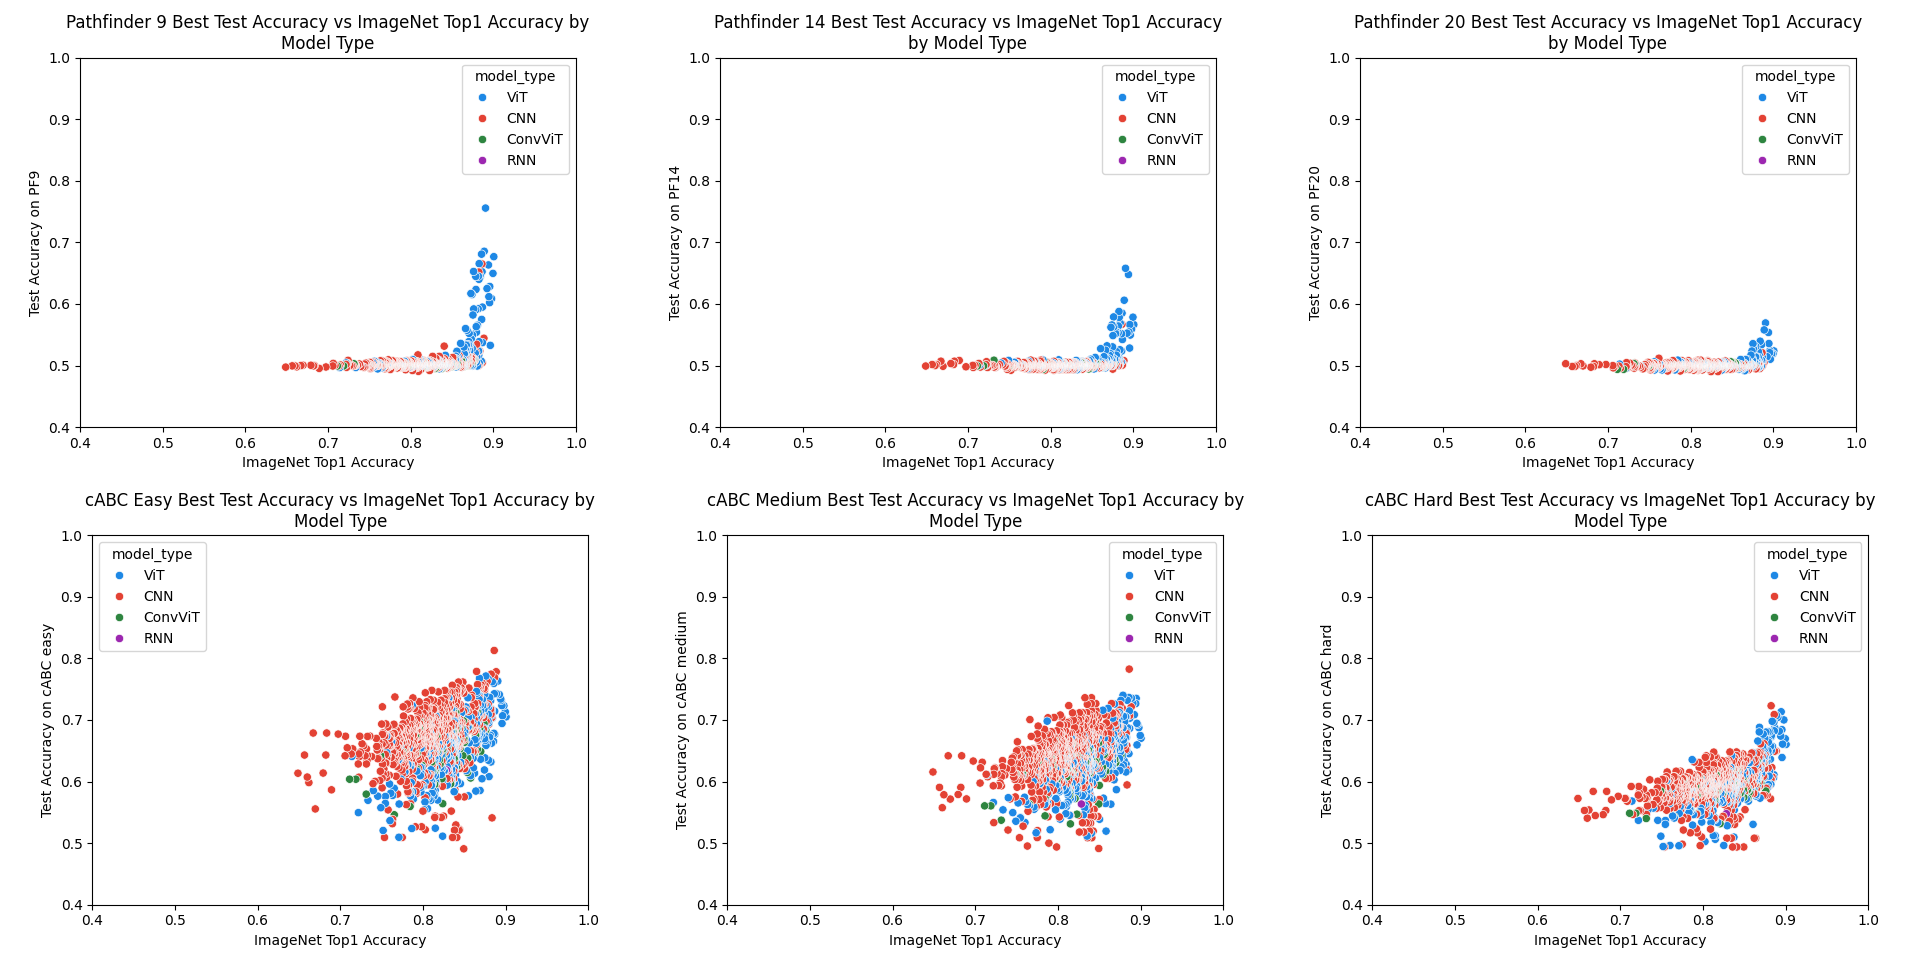
\includegraphics[width=\textwidth]{Combined Test Graphs.png}
\caption{When breaking down model performances across the Pathfinder and cABC tasks, model performance in aggregate (p = 1259) noticeably decreased as the difficulty of the task – an indication of the distance in the long-range reasoning required for the task – increased. This pattern is most apparent in the Pathfinder task, which also saw better-than-random performance exclusively at those models which had the highest ImageNet accuracy, here using Top1 performance as a loose proxy for model size. cABC showed broader above-chance performance that nevertheless degraded with difficulty.} 
\label{Zoo-Results}
\end{figure*}

Across both tasks, model performance in aggregate decreased as the difficulty of the particular task increased. However, these effects were much more pronounced in the Pathfinder task, with linear probes attached to pre-trained models being capable of significantly above-random performance in the lowest Pathfinder difficulty but all models falling to near-random performance in the highest difficulty. cABC saw better model performance overall, though with some dropoff as difficulty increased.

Notably, models using traditional convolutional networks were uniformly weak on the Pathfinder task, indicating that convolutional neural networks broadly struggle to encode long-range dependencies. Success was instead found in transformer-based architectures, where self-attention successfully encoded low-distance dependencies, though dropping off as the distance increased.

A significantly weaker version of this trend can be observed in the cABC task, where CNN-based models show the sharpest drop-off in performance as the difficulty increases. However, CNNs acquit themselves well compared to Pathfinder, perhaps indicating that the long-range dependencies in the cABC task can be learned more easily than Pathfinder.

Overall, the use of linear probing shows that models can struggle to -- or fail entirely to -- encode long-range spatial information when trained on broader computer vision tasks, rather than the contested observation that current models cannot be trained to extract them at all.

% Figure~\ref{sample-figure}. If necessary, leave extra white space at
% the bottom of the page to avoid splitting the figure and figure
% caption. You may float figures to the top or bottom of a column, or
% set wide figures across both columns.

\section{Conclusion}

Despite impressive performance from ViTs and concerns about LRA (Miralles{-}Gonz{\'{a}}lez, 2025), lackluster model performance on these tasks gives reason to believe that representational successes in computer vision are insufficient for or distinct from the representational requirements of long-range visual reasoning. Future architectures may well need specific mechanisms for spatial reasoning over distance, rather than general recognition capacity. 


\section{Acknowledgments (camera-ready version only)}
Please refrain from adding acknowledgments to the double-blind version to protect anonymity. Include acknowledgments \textbf{only} in the final accepted version of the manuscript. 

\nocite{Serre2018a}
\nocite{Serre2018b}
\nocite{LRA}
\nocite{Amos}
\nocite{Wightman}
\nocite{Dosovitskiy}
\nocite{Miralles}
\nocite{Houtkamp}
\nocite{Gu}

% \nocite{ChalnickBillman1988a}
% \nocite{Feigenbaum1963a}
% \nocite{Hill1983a}
% \nocite{OhlssonLangley1985a}
% % \nocite{Lewis1978a}
% \nocite{Matlock2001}
% \nocite{NewellSimon1972a}
% \nocite{ShragerLangley1990a}


\newpage


\bibliographystyle{ccn_style}

\setlength{\bibleftmargin}{.125in}
\setlength{\bibindent}{-\bibleftmargin}

\bibliography{ccn_style}


\end{document}
